\chapter{Introduction}

\section{Motor Controls}

\subsection{Overview}

The motor control subsystem governs the movement of the vehicle and is implemented within a single software file. It receives input from the pathfinding algorithm and translates this into control signals for the two on-board motors. The original motors are retained, and no modifications to the chassis are required.

\subsection{Hardware Architecture}

The motor control subsystem consists of two DC motors: a rear-mounted drive motor responsible for propulsion and a front-mounted motor used for steering via wheel pivoting. This configuration is retained from the original chassis design, avoiding physical modifications and ensuring compliance with project requirements on chassis dimensions. Maintaining the existing layout also reduces mechanical complexity and ensures compatibility with the pre-defined mounting structure.

Motor actuation is achieved using an L298N Dual H-Bridge Motor Driver Module, which provides an interface between the ESP32 microcontroller and the motors. The driver enables bidirectional control of each motor using an H-bridge configuration, allowing both forward and reverse operation.

The ESP32 supplies control signals to the driver through four digital input pins, which determine the direction of rotation for each motor. These input pins are arranged in pairs, with IN1 and IN2 controlling the steering motor, and IN3 and IN4 controlling the drive motor. By setting one pin in each pair high while the other is low, the polarity of the voltage applied to each motor is controlled.

The mapping between ESP32 GPIO pins and motor driver inputs is shown in Figure~\ref{fig:gpio_mapping}. In the implemented control scheme, each GPIO pin is associated with a specific vehicle movement command. Before a new command is issued, all motor control pins are driven low, ensuring that only one control signal is active at a time. This simplifies direction control and prevents conflicting input states from being applied to the motor driver.

\begin{figure}[h]
  \centering
  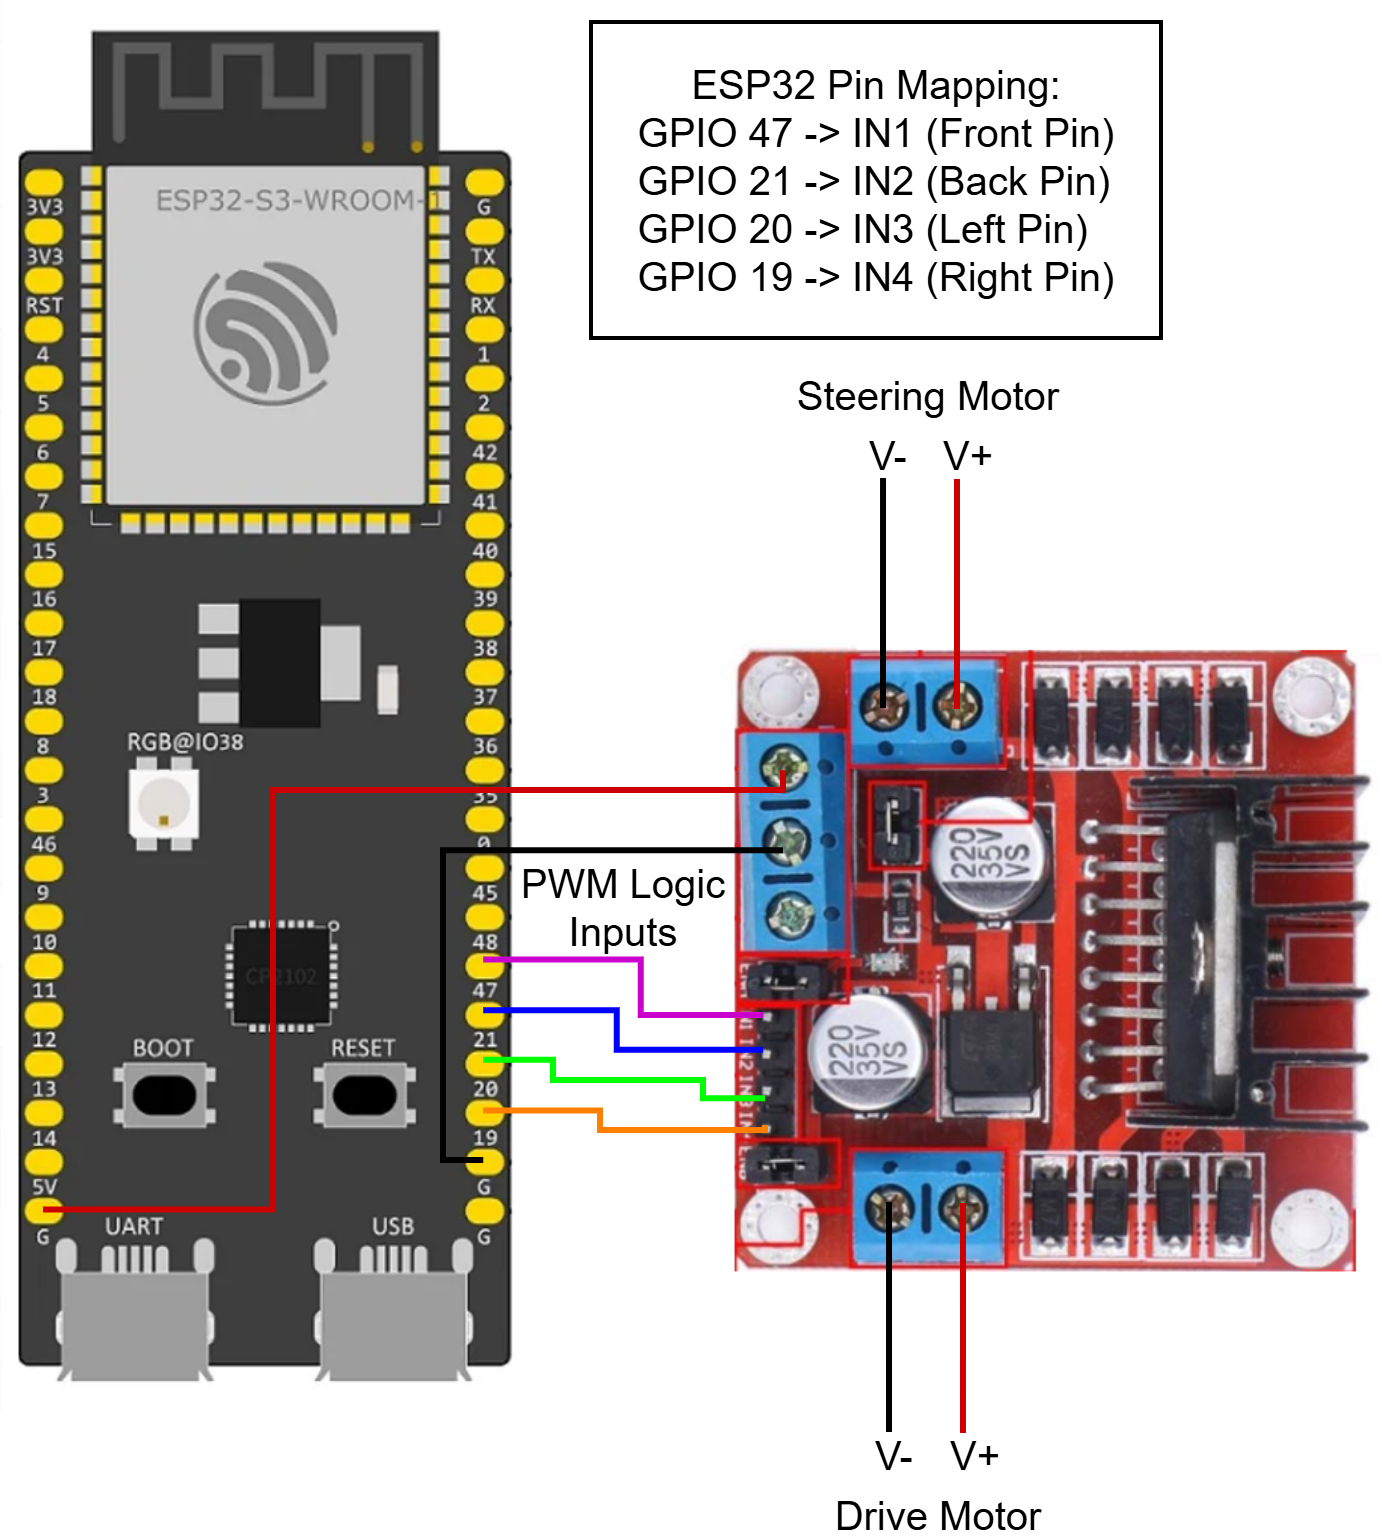
\includegraphics[width=0.7\textwidth]{images/MotorDriverPinsV2.png}
  \caption{Mapping between ESP32 GPIO pins and motor driver inputs}
  \label{fig:gpio_mapping}
\end{figure}

Speed control is achieved using Pulse Width Modulation (PWM) signals generated by the ESP32 and applied to the enable pins of the driver. As the control signals are digital, the amplitude of the PWM signal remains constant, and motor speed is regulated by adjusting the duty cycle.

The L298N module is powered separately from the ESP32 logic supply, providing sufficient current to drive the motors. While the ESP32 operates at 3.3~V logic levels, the driver is compatible with these signals, enabling direct interfacing without additional level shifting circuitry.

\subsection{Control Logic}

The motor control system is implemented using four PWM channels, each corresponding to one input pin of the motor driver (IN1--IN4). At system initialisation, the \texttt{Motors\_Init()} function is called, configuring all PWM signals with a duty cycle of 0\%, ensuring that no motors are driven by default.

When the \texttt{Motors\_Apply()} function is invoked, control inputs from the pathfinding module are used to update the duty cycles of the relevant PWM channels. The order of operations is illustrated in Figure~\ref{fig:control_flow}.

\begin{figure}[h]
  \centering
  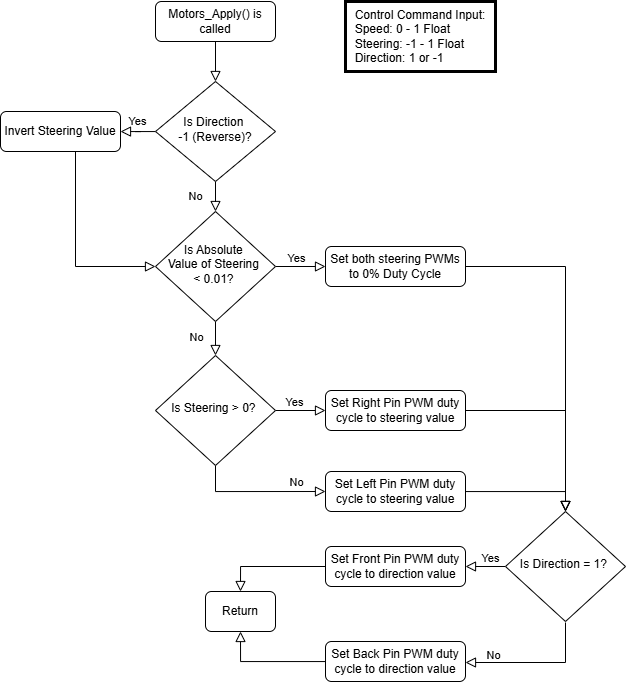
\includegraphics[width=0.7\textwidth]{images/MotorLogic.png}
  \caption{Motor control logic flow}
  \label{fig:control_flow}
\end{figure}

A non-zero duty cycle is applied only to the PWM channel corresponding to the desired direction of motion, while the complementary channel in the input pair remains at 0\%. This ensures that only one control signal is active for each motor at any time, preventing conflicting inputs from being applied to the motor driver.

Steering and propulsion are handled independently. The steering input determines which of the steering-related PWM channels is activated and to what duty cycle, while the direction input determines which propulsion-related channel is driven. This structure allows high-level motion commands to be translated directly into low-level motor control signals.

The control logic begins by evaluating the direction input. If the direction is negative (reverse), the sign of the steering value is inverted. This is required because the pathfinding algorithm defines steering relative to the forward-facing orientation of the vehicle; when reversing, the steering response must be inverted to achieve the intended motion.

Following this, the steering value is evaluated to configure the steering PWM outputs. To prevent unintended drift caused by very small floating-point values, a deadband is applied. If the magnitude of the steering input is below 0.01, both steering PWM channels are set to a duty cycle of 0\%. If the value is positive, the vehicle steers right; if negative, it steers left.

Finally, propulsion is configured by evaluating the direction input and applying the speed value to the corresponding PWM channel. This step is performed after steering configuration to ensure that the wheels are correctly oriented before motion begins. This ordering reduces the likelihood of incorrect movement if an interrupt occurs during execution of the \texttt{Motors\_Apply()} function.

\subsection{Software Implementation}

The motor control subsystem is structured as a modular interface consisting of three primary functions: \texttt{Motors\_Init()}, \texttt{Motors\_Apply()}, and \texttt{Motors\_Stop()}. This structure provides a clear abstraction layer between the motor control logic and the higher-level finite state machine.

The \texttt{Motors\_Init()} function is responsible for configuring the PWM channels used to drive the motor driver inputs. PWM generation and duty cycle control are implemented using the ESP32 LEDC library. All PWM channels are initialised with a duty cycle of 0\%, ensuring that the motors remain inactive on system startup.

The \texttt{Motors\_Apply()} function implements the control logic described in the previous section and serves as the main interface for motor actuation. It receives speed, steering, and direction inputs from the pathfinding module and translates these into PWM duty cycles applied to the motor driver inputs.

Input validation is performed within this function to ensure robust operation. Speed and steering values are constrained to the range [-1, 1], with out-of-range inputs clamped while preserving their original sign. The direction input is expected to be either -1 or 1; invalid values default to forward motion. This behaviour is intentionally chosen to prioritise forward displacement in the event of unexpected pathfinding outputs, maximising progress through the course while minimising reverse motion that does not contribute to overall advancement.

The function updates the PWM outputs by mapping validated input values directly to duty cycles, ensuring that only the channel corresponding to the intended direction of motion is active at any given time. This maintains consistency with the control scheme described previously and prevents conflicting motor commands.

The \texttt{Motors\_Stop()} function provides a simple mechanism to halt all motor activity by setting the duty cycle of all PWM channels to 0\%. This function is used both during testing and as a safety mechanism during operation.

\subsection{Testing}

The motor control subsystem was validated using a dedicated test driver, which repeatedly invoked the \texttt{Motors\_Apply()} function with predefined input values. These inputs were selected to cover both standard operating conditions and edge cases near decision thresholds within the control logic.

Each test case was executed on the physical hardware for a duration of 2 seconds, followed by a 0.5 second pause. During this pause, the \texttt{Motors\_Stop()} function was called, ensuring that both motion and stopping behaviour were verified. This approach allowed the response of the motors to be clearly observed for each input condition.

Test cases included nominal inputs, such as full forward motion and directional steering, as well as edge cases involving small steering magnitudes and direction changes. Due to the physical nature of the system, results were validated through observation of motor behaviour, confirming that the vehicle responded in accordance with the expected direction and speed.

The test suite was structured into four categories: normal operation, boundary conditions on speed, boundary conditions on steering, and extreme input values. Normal tests verified expected behaviour for typical motion commands, including forward, reverse, and combined steering inputs. Boundary tests evaluated system behaviour at and beyond defined input limits (e.g.\ $\pm1.0$), ensuring stable operation near decision thresholds. Extreme tests used significantly out-of-range values to confirm that the system remained stable and did not produce undefined behaviour.

A representative subset of test cases is shown in Table~\ref{tab:motor_tests}, with the full test suite provided in Appendix~A.

\begin{table}[h]
\centering
\begin{tabular}{|l|l|p{4cm}|p{4cm}|c|}
\hline
\textbf{Test Name} & \textbf{Input Value} & \textbf{Expected Result} & \textbf{Actual Result} & \textbf{Passed?} \\
\hline

Forward Only & [0.9f, 0.0f, 1] & Car drives straight forward, 75\% speed & Car drives straight forward, 75\% speed & Yes \\
\hline

Left Only & [0.0f, -0.9f, 1] & Front wheels turn left at a medium rate & Front wheels turn left at a medium rate & Yes \\
\hline

Reverse Left & [0.0f, 0.9f, -1] & Car reverses and turns left at medium rate & Car reverses and turns left at medium rate & Yes \\
\hline

Forward Speed Edge Over & [1.01f, 0.0f, 1] & Car drives straight forward, full speed & Car drives straight forward, full speed & Yes \\
\hline

Forward \& Left Under & [0.99f, -0.99f, 1] & Car drives forward, turning left, almost full speed & Car drives forward, turning left, almost full speed & Yes \\
\hline

Extreme Back \& Right & [20.0f, -20.0f, -1] & Car reverses right at full speed & Car reverses right at full speed & Yes \\
\hline

\end{tabular}
\caption{Motor control test results}
\label{tab:motor_tests}
\end{table}

\section{Path Planning}

\subsection{Overview}

\todo[inline, color=red!40]{Need to add stuff on when an obstacle is too close it starts reversing when thats implemented.}

The path planning subsystem is responsible for converting sensor data into motion commands for the vehicle. Unlike a map-based planner, this implementation uses an artificial potential field (APF) approach, in which the vehicle is guided by a combination of attractive and repulsive influences derived from the sensors. The resulting heading and speed are then passed into the motor control subsystem.

This method was chosen because it is compact, computationally efficient, and allows for a small non complete map to be used. The path planning logic operates directly on the inputs from the infrared and distance sensors along with the IMU data. By using continuous sensor feedback, the vehicle is able to react dynamically to changes in the environment while maintaining smooth motion.

\subsection{Sensor Interpretation and Field Construction}

The path planning algorithm uses four infrared (IR) sensors positioned around the vehicle, together with a front-facing time-of-flight (ToF) distance sensor and an inertial measurement unit (IMU). The IR readings are first clamped to prevent invalid values from influencing the navigation logic. These readings are then grouped into left, right, front, and rear loads, allowing the vehicle to estimate its location relative to nearby walls.

A measured wall heading is computed using the relationship:

\[\theta_{wall} = \arctan2(L - R, F - B)\]

where $L$ and $R$ represent the combined left and right sensor loads, and $F$ and $B$ represent the combined front and rear loads. This heading is wrapped to the range of $[-180^\circ, 180^\circ]$ to ensure the path planning outputs are possible for the vehicle to achieve.

\todo[inline, color=red!40]{This section should be updated after IMU integration is finalized.}

During initialisation, the subsystem stores an \emph{original wall heading}, which acts as a stable reference direction. This reference is first established when the ToF sensor reports a valid distance measurement. Once initialised, the stored heading is updated each cycle using the current IR balance and distance information, allowing the reference direction to adapt gradually, allowing the system to adapt to changing conditions.
\subsection{Control Logic}

The navigation decision is based on the combination of attractive and repulsive fields. The attractive component encourages the vehicle to move in the direction of the stored wall heading, which acts as the intended course direction. Its magnitude is scaled according to the measured front distance, meaning that the vehicle is encouraged to move more strongly when there is sufficient space ahead.

Repulsive forces are generated from the IR sensor imbalance. These forces oppose proximity to nearby tape or obstacles and are calculated using the difference between the left and right sensor loads, as well as the front and rear loads. The repulsive field is then combined with the attractive field to produce a resultant vector representing the desired direction of travel.

The final heading is calculated from this resultant vector using:

\[\theta_{desired} = \arctan2(F_y, F_x)\]

where $F_x$ and $F_y$ are the horizontal and vertical components of the combined field. This approach allows the vehicle to balance course-following behaviour with obstacle avoidance in a single control step.

Speed is estimated from the magnitude of the resultant field and then adjusted according to environmental risk. Motion is reduced when the vehicle is close to a wall or obstacle, it is also reduced when the IR sensors indicate a strong tape danger signal. In addition, if the repulsive component becomes large, the maximum speed is capped to reduce oscillation and improve stability. This produces smoother behaviour in confined or ambiguous sections of the course.

To prevent abrupt changes in motion, both heading and speed are filtered using simple temporal smoothing by interpolating the new output with the previous. The new command is interpolated with the previous output, which reduces jitter and helps the vehicle maintain stable motion across successive control cycles.

\subsection{Software Implementation}

The path planning subsystem is implemented through two primary functions: \texttt{apf\_navigation\_init()} and \texttt{apf\_navigation\_compute()}. A third function, \texttt{apf\_navigation\_to\_control()}, converts the resulting navigation command into the format required by the motor control subsystem.

The \texttt{apf\_navigation\_init()} function resets the internal state variables used by the planner. These include the stored wall heading, a validity flag indicating whether the reference heading has been established, and the previous heading and speed values used for smoothing. Initialising these values ensures that the first navigation cycle begins from a known state.

The \texttt{apf\_navigation\_compute()} function contains the main APF logic. It receives sensor data, validates and clamps the inputs, computes the attractive and repulsive components, and produces a desired heading and speed. Internal memory is updated at the end of each call so that the next iteration can make use of the previous output. This stateful design is important because it provides continuity between control cycles and improves navigation stability.

The \texttt{apf\_navigation\_to\_control()} function maps the APF output into low-level drive commands. The heading is normalised to a steering range by dividing it by $45^\circ$ and clamping the result to $[-1,1]$. The speed value is also constrained to $[0,1]$. The direction output is fixed to forward motion, meaning that the planner is designed primarily for continuous forward navigation rather than reversing manoeuvres.

This separation between navigation and actuation provides a clear abstraction layer. The path planner determines \emph{where} the vehicle should move, while the motor control subsystem determines \emph{how} that motion is physically applied to the motors.

\subsection{Behavioural Characteristics}

The implemented APF strategy provides several useful behaviours. The vehicle tends to follow a stable course when the surroundings are consistent, because the original wall heading acts as a persistent directional reference. When the environment changes, the repulsive field helps prevent collisions or tape violations by steering the vehicle away from local hazards. The smoothing stage then prevents the output from changing too abruptly, which is particularly beneficial when sensor readings fluctuate between adjacent control cycles.

The use of a distance-based speed reduction also improves safety. When the vehicle approaches a wall or obstacle, the planner automatically slows the vehicle down, giving the steering system more time to respond. Similarly, strong IR activity near the tape causes the vehicle to reduce speed, lowering the likelihood of overshooting the course boundary.

Overall, the path planning subsystem provides a lightweight and reactive navigation method that is well matched to the available sensors and embedded processing platform. Its continuous control structure allows the vehicle to maintain progress while dynamically adapting to local obstacles and course constraints.

\section{Policies and Procedures Document}

\subsection{Version Control and Code Management}
All project code was managed using a distributed version control system hosted on GitHub. The project was developed within a Dev Container environment, ensuring that all team members worked with identical toolchains and dependencies.
Each team member developed features on individual branches, reducing the risk of conflicts and enabling parallel progress. Changes were merged into the main branch only after testing and verification had been demonstrated to the group.
Frequent commits were encouraged to ensure that progress was continuously recorded and recoverable. This also enabled rollback to previously stable versions in the event of errors or regressions.
Subsystem interfaces were defined prior to development, specifying expected input and output formats. This allowed consistent integration between components and ensured a uniform function naming convention across the codebase.

\subsection{Code Review Practices}
Code reviews were conducted informally within the group prior to merging changes into the main branch. Reviews were performed after testing had been completed, ensuring that both functionality and code quality were assessed.
Team members evaluated each other’s work to identify potential issues, improve readability, and maintain consistency in coding style. Attention was given to critical components such as motor control and pathfinding logic, where incorrect behaviour could significantly impact system performance.
This collaborative review process contributed to improved code reliability and reduced the likelihood of integration issues.

\subsection{Task Allocation and Monitoring}
Tasks were allocated based on subsystem responsibilities, including motor control, sensor integration, state machine design, and pathfinding. This allowed each team member to focus on a specific area while maintaining clear ownership of their component.
Hardware integration was treated as a shared responsibility and was carried out during the later stages of development, once most software components had been implemented.
Progress was monitored through weekly group meetings, where updates were shared and blockers identified. This ensured that issues were addressed early and that workload remained balanced across the team.

\subsection{Risk Management and Resilience}
To mitigate risks associated with delays or unforeseen issues, several measures were implemented. The use of version control ensured that all work was centrally accessible and protected against data loss.
Clear documentation of subsystem interfaces allowed components to be understood and modified by multiple team members, reducing dependency on any single individual.
Frequent commits ensured that development progress was regularly checkpointed, enabling recovery in the event of disruption. Regular integration and testing further ensured that the system remained functional throughout development, reducing the risk of late-stage failures.
